\section{Recurrent Multi-Object Tracking with Self-Attention}
%\vspace{-3mm}
\label{sec:mohart_method}

\begin{figure}
	\centering
	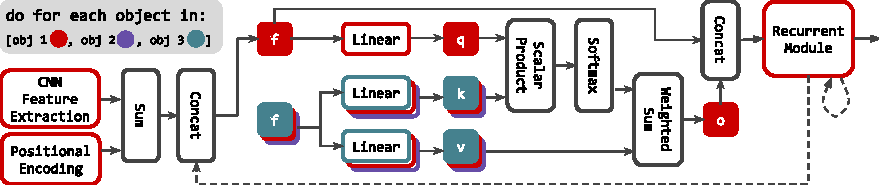
\includegraphics[width=\linewidth]{figures/MOHART/sab.pdf}
	\caption{
		The relational reasoning module in \Gls{MOHART} based on multi-headed self-attention. Here, we show the computation of the interaction of the red object with all other objects. Object representations $f_{t,m}$ are computed using visual features, positional encoding and the hidden state from the recurrent module. These are linearly projected onto keys (k), queries (q), and values (v) to compute a weighted sum of interactions between objects, yielding an interaction vector $o_{t,m}$. Subscripts $t, m$ are dropped from all variables for clarity of presentation, so is the splitting into multiple heads.
	}
	\label{fig:sab}
\end{figure}

This section describes the model architecture in \cref{fig:teaser}. We start by describing the \glsreset{HART}\gls{HART} algorithm of \Cref{ch:hart}, and then follow with an extension of \gls{HART} to tracking multiple objects, where multiple instances of \gls{HART} communicate with each other using multi-headed attention to facilitate relational reasoning. We also explain how this method can be extended to trajectory prediction instead of just tracking. 

\subsection{Hierarchical Attentive Recurrent Tracking (\textsc{hart})}
\vspace{-3mm}
%\vspace{-.5em}
%\paragraph{Hierarchical Attentive Recurrent Tracking (\textsc{hart})}
\textsc{Hart} is an attention-based recurrent algorithm, which can efficiently track single objects in a video.
It uses a spatial attention mechanism to extract a \textit{glimpse} $\bg_t$, which corresponds to a small crop of the image $\bxt$ at time-step $t$, containing the object of interest.
This allows it to dispense with the processing of the whole image and can significantly decrease the amount of computation required.
\Gls{HART} uses a \gls{CNN} to convert the glimpse $\bg_t$ into features $\mathbf{f}_t$, which then update the hidden state $\mathbf{h}_t$ of a \gls{LSTM} core.
The hidden state is used to estimate the current bounding-box $\mathbf{b}_t$, spatial attention parameters for the next time-step $\ba_{t+1}$, as well as object appearance.
Importantly, the recurrent core can learn to predict complicated motion conditioned on the past history of the tracked object, which leads to relatively small attention glimpses---contrary to \gls{CNN}-based approaches \citep{Held2016goturn,Valmadre2017}, \gls{HART} does not need to analyse large regions-of-interest to search for tracked objects.
In the original paper, \textsc{hart} processes the glimpse with an additional ventral and dorsal stream on top of the feature extractor. Early experiments have shown that this does not improve performance on the MOTChallenge dataset, presumably due to the oftentimes small objects and overall small amount of training data. 
Further details are provided in \Cref{sec:mohart_architecture_details}.

	The algorithm is initialised with a bounding-box\footnote{We can use either a ground-truth bounding-box or one provided by an external detector; the only requirement is that it contains the object of interest.} $\mathbf{b}_1$ for the first time-step, and operates on a sequence of raw images $\bx_{1:T}$.
	For time-steps $t\geq2$, it recursively outputs bounding-box estimates for the current time-step and predicted attention parameters for the next time-step. The performance is measured as intersection-over-union (IoU) averaged over all time steps in which an object is present, excluding the first time step.

Although \gls{HART} can track arbitrary objects, it is limited to tracking one object at a time.
While it can  be deployed on several objects in parallel, different \gls{HART} instances have no means of communication.
This results in performance loss, as it is more difficult to identify 
occlusions, ego-motion and object interactions.
Below, we propose an extension of \gls{HART} which remedies these shortcomings.

\subsection{Multi-Object Hierarchical Attentive Recurrent Tracking (\textsc{mohart})}
\vspace{-3mm}
%\vspace{-.5em}
%\paragraph{Multi-Object Hierarchical Attentive Recurrent Tracking (\textsc{mohart})}
Multi-object support in \gls{HART} requires the following modifications.
Firstly, in order to handle a dynamically changing number of objects, we apply \gls{HART} to multiple objects in parallel, where all parameters between \gls{HART} instances are shared. 
We refer to each \gls{HART} instance as a \textit{tracker}.
Secondly, we introduce a presence variable $p_{t,m}$ for object $m$.
It is used to mark whether an object should interact with other objects, as well as to mask the loss function (described in \Cref{ch:hart}) for the given object when it is not present.
In this setup, parallel trackers cannot exchange information and are conceptually still single-object trackers, which we use as a baseline, referred to as \gls{HART} (despite it being an extension of the original algorithm).
Finally, to enable communication between trackers, we augment \gls{HART} with an additional step between feature extraction and the \gls{LSTM}.

For each object, a glimpse is extracted and processed by a CNN (see \cref{fig:teaser}). Furthermore, spatial attention parameters are linearly projected on a vector of the same size and added to this representation, acting as a positional encoding. This is then concatenated with the hidden state of the recurrent module of the respective object (see \cref{fig:sab}). Let $\mathbf{f}_{t, m}$ denote the resulting feature vector corresponding to the m$^\mathrm{th}$ object, and let $\mathbf{f}_{t, 1:M}$ be the set of such features for all objects.
Since different objects can interact with each other, it is necessary to use a method that can inform each object about the effects of their interactions with other objects.
Moreover, since features extracted from different objects comprise a set, this method should be permutation-equivariant,\ie the results should not depend on the order in which object features are processed.
Therefore, we use the multi-head self-attention block (\textsc{sab}, \citet{Lee2019set}), which is able to account for higher-order interactions between set elements when computing their representations. %, thereby allowing rich information exchange, and it can do so in a permutation-equivariant manner.
Intuitively, in our case, \textsc{sab} allows any of the trackers to query other trackers about attributes of their respective objects,\eg distance between objects, their direction of movement, or their relation to the camera.
This is implemented as follows,
\begin{align}
Q &= W_q \mathbf{f}_{1:M} + b_q\,, \qquad K = W_k \mathbf{f}_{1:M} + b_k\,, \qquad V = W_v \mathbf{f}_{1:M} + b_v \label{eq:projection}\,,\\
&\hspace{1.5em} O_i = \operatorname{softmax}\left( Q_i K_i^T \right) V_i\,, \qquad i=1,\dots,H\,, \label{eq:att}\\
&\hspace{7em} o_{1:M} = O = \operatorname{concat}(O_i,\dots,O_H)\,, \label{eq:multihead}
\end{align}
where $o_m$ is the output of the relational reasoning module for object $m$. Time-step subscripts are dropped to decrease clutter.
In Eq. \ref{eq:projection}, each of the extracted features $\mathbf{f}_{t,m}$ is linearly projected into a triplet of key $\mathbf{k}_{t,m}$, query $\mathbf{q}_{t,m}$ and value $\mathbf{v}_{t,m}$ vectors. Together, they comprise $K, Q$ and $V$ matrices with $M$ rows and $d_q, d_k, d_k$ columns, respectively.
$K, Q$ and $V$ are then split up into multiple heads $H \in \mathbb{N}_+$, which allows to query different attributes by comparing and aggregating different projection of features.
Multiplying $Q_iK_i^T$ in Eq. \ref{eq:att} allows to compare every query vector $\mathbf{q}_{t,m,i}$ to all key vectors $\mathbf{k}_{t,1:M,i}$, where the value of the corresponding dot-products represents the degree of similarity.
Similarities are then normalised via a $\operatorname{softmax}$ operation and used to aggregate values $V$.
Finally, outputs of different attention heads are concatenated in Eq. \ref{eq:multihead}.
\textsc{Sab} produces $M$ output vectors, one for each input, which are then concatenated with corresponding inputs and fed into separate \gls{LSTM}s for further processing, as in \gls{HART}---see \cref{fig:teaser}.


\begin{figure}[t!]%
	\centering
	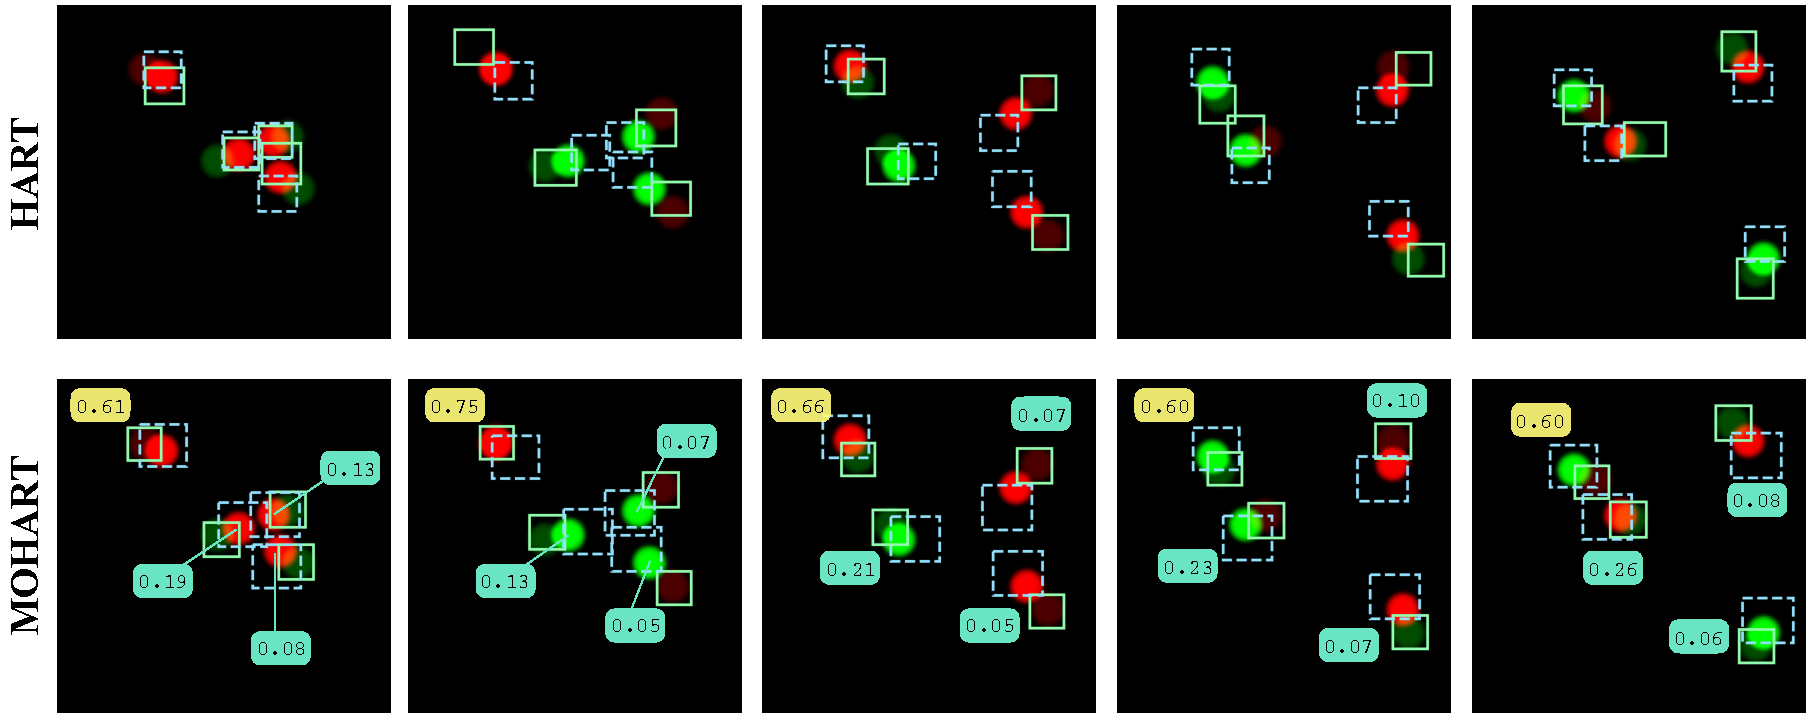
\includegraphics[width=0.99\textwidth]{figures/MOHART/mot_proel.pdf}
	% \vspace{-3mm}
	\caption{
		A scenario constructed to be impossible to solve without relational reasoning. Circles of the same colour repel each other, circles of different colour attract each other. Crucially, each circle is randomly assigned its identity in each time step. Hence, the algorithm can not infer the forces exerted on one object without knowledge of the state of the other objects in the current time step. The forces in this scenario scale with $1/\sqrt{r}$ and the algorithm was trained to predict one time step into the future. \textsc{hart} (top) is indeed unable to predict the future location of the objects accurately. The achieved average IoU is $47\%$, which is only slightly higher than predicting the objects to have the same position in the next time step as in the current one ($34\%$). Using the relational reasoning module, \textsc{mohart} (bottom) is able to make meaningful predictions ($76\%$ IoU). The numbers in the bottom row indicate the self-attention weights from the perspective of the top left tracker (yellow number box). Interestingly, the attention scores have a strong correlation with the interaction strength (which scales with distance) without receiving supervision.
		\vspace{-3mm}
	}
	\label{fig:toy2}
\end{figure}


\Gls{MOHART} is trained fully end-to-end, contrary to other tracking approaches. % \citep{Zhang2008,Milan2014,bae2017confidence,keuper2018motion}.
It maintains a hidden state, which can contain information about the object's motion. One benefit is that in order to predict future trajectories, one can simply feed black frames into the model. Our experiments show that the model learns to fall back on the motion model captured by the \gls{LSTM} in this case. 


\subsection{Multi-Object Baselines}

\vspace{-.5em}
\paragraph{\Gls{MLP}} In this version, the representations of all objects are concatenated and fed into a fully connected layer followed by ELU activations. The output is then again concatenated to the unaltered feature vector of each object. This concatenated version is then fed to the recurrent module of \gls{HART}. This way of exchanging information allows for universal function approximation (in the limit of infinite layer sizes) but does not impose permutation invariance.


\vspace{-.5em}
\paragraph{DeepSets} Here, the learned representations of the different objects are summed up instead of concatenated and then divided by total number of objects. 
% This has lower capacity than the \gls{MLP} version. 
This is closely related to DeepSets \citep{Zaheer2017} and allows for universal function approximation of all permutation invariant functions \citep{Wagstaff2019}.

\vspace{-.5em}
\paragraph{Max-Pooling} Similar to DeepSets, but using max-pooling as the permutation invariant operation. This way of exchanging information is used, e.g., by \citet{Alahi2016social} who predict future pedestrian trajectories from ground truth tracklets in coordinate space.


